\chapter{Theoretische Grundlagen und Stand der Forschung}
\label{chapter:related_work}


\section{Fahrassistenzsysteme als sicherheitskritische
Mensch-Maschine-Interaktion}
\label{sec:fas_sicherheitskritisch}
Dieses Unterkapitel betrachtet grundlegende theoretische Modelle und Begriffe, welche in der Literatur \cite{Geisler_hci2021} identifiziert wurden und die besonderen Herausforderungen an Gestaltungslösungen in diesem Zusammenhang aufzeigen.

\subsection{Fahraufgaben}
\label{subsec:fahraufgabe}
Zur besseren Abgrenzung der Aufgabenbereiche von Fahrer*innen und Assistenzsystemen in einem Fahrzeug, wird an dieser Stelle zunächst erstgenannter definiert. Geisler \cite{Geisler_hci2021} nennt den sicheren Transport vom Ausgangs- zum Zielort als Haupt- oder Primäraufgabe der Fahrer*innen und verweist auf unterstützende Aufgaben, die zur Erfüllung der primären Aufgabe notwendig sind.

\begin{table}[ht]
\centering
\caption{Einteilung von Fahraufgaben aus Sicht der Fahrer*innen}
\label{tab:fahraufgaben}

\begin{tabular}{|p{0.29\textwidth}|p{0.34\textwidth}|p{0.29\textwidth}|}
\hline
\textbf{Primäre Aufgabe} &
\textbf{Sekundäre Aufgabe} &
\textbf{Tertiäre Aufgabe}
\\ \hline

Transport der Personen beziehungsweise Güter &
Zusätzliche fahraufgabenbezogene Tätigkeiten abhängig von primärer Fahraufgabe &
Nicht verbunden mit der Fahraufgabe
\\ \hline

Navigation: Planung der Route &
Interaktion mit anderen Verkehrsteilnehmenden: blinken, hupen, Handzeichen geben &
Komfort: Klimaanlage, Sitzheizung, Panoramadach, Massagesitz
\\ \hline

Führung: Festlegung von Soll-Geschwindigkeit und Kurs (Fahrspur), beides in der Regel situationsabhängig &
Reaktionen auf die Umwelt: Steuerung von Licht, Scheibenwischer, Heckscheibenheizung, Gangwechsel &
Unterhaltung, Information: Radio und Mediaplayer, Verkehrsinformationen
\\ \hline

Stabilisierung: Längs- und Querdynamik, das heißt Beschleunigen/Bremsen und Lenken &
&
Kommunikation: Telefon, Kurznachrichten
\\ \hline

Notwendig zur Erreichung des Ziels &
Erreichung des Ziels auch ohne diese Tätigkeiten möglich, aber mit erheblichen Einschränkungen &
Erreichung des Ziels auch ohne diese Tätigkeiten möglich
\\ \hline

Teilweise extrem zeitkritisch (Stabilisierungsaufgabe) &
Geringe zeitliche Anforderungen &
Keine zeitlichen Anforderungen
\\ \hline
\end{tabular}

\medskip
{\footnotesize Quelle: Tabelle inhaltlich übernommen aus
\cite[S.~365]{Geisler_hci2021}.}
\end{table}

Tabelle \ref{tab:fahraufgaben} zeigt die an Geiser \cite{Geiser1985}, Bubb \cite{bubb2015automobilergonomie} und Donges \cite{donges2015fahrerverhaltensmodelle} angelehnte Einteilung von Fahraufgaben aus Sicht der Fahrer*innen nach Darstellung von Geisler \cite{Geisler_hci2021}. Es wird an dieser Stelle deutlich, dass der große Aufgabenbereich der fahrzeugführenden Person mit teilweise kokurrierenden Aufgaben, für eine selektiv arbeitende menschlichen Aufmerksamkeit \cite{Broadbent1958} eine große Herausforderung darstellt, weswegen eine Priorisierung der Unterstützungstätigkeiten für die Aufgaben obligatorisch erscheint. Geisler \cite{Geisler_hci2021} konstatiert, dass im Hinblick auf Sicherheitsaspekte zudem darauf zu achten sei, dass bei den primären Aufgaben die Beherrschbarkeit der Funktionen und bei tertiären Aufgaben eine möglichst geringe Ablenkung sicherzustellen sind. Die Empfehlungen für die sekundären Aufgaben seien als Kombination der zuletzt genannten Empfehlungen zu verstehen, so der Forscher \cite{Geisler_hci2021}. 

Für diese Masterarbeit sind die Erkenntnisse zentral, da Assistenzsysteme zunächst der Aufgabenart, bei der sie die fahrzeugführende Person unterstützen, zugeordnet werden sollten. Aufbauend darauf, sollten die zuletzt genannten Empfehlungen auch für ein Onboarding einer solchen Assistenzfunktion Beachtung finden, indem bestimmte Informationen, die zur sicheren Erledigung der Aufgabenart zentral sind, priorisiert werden.    

\subsection{Fahrverhalten}
\label{subsec:ausgewaehlte_assistenzfunktion}
Das Fahrverhalten der fahrzeugführenden Person ist ein weiterer grundlegender Aspekt im Kontext dieser Forschungsarbeit, der eng mit dem Erkenntnissen von Kapitel \ref{subsec:fahraufgabe} verknüpft ist. 

\begin{figure}[ht]
    \centering
    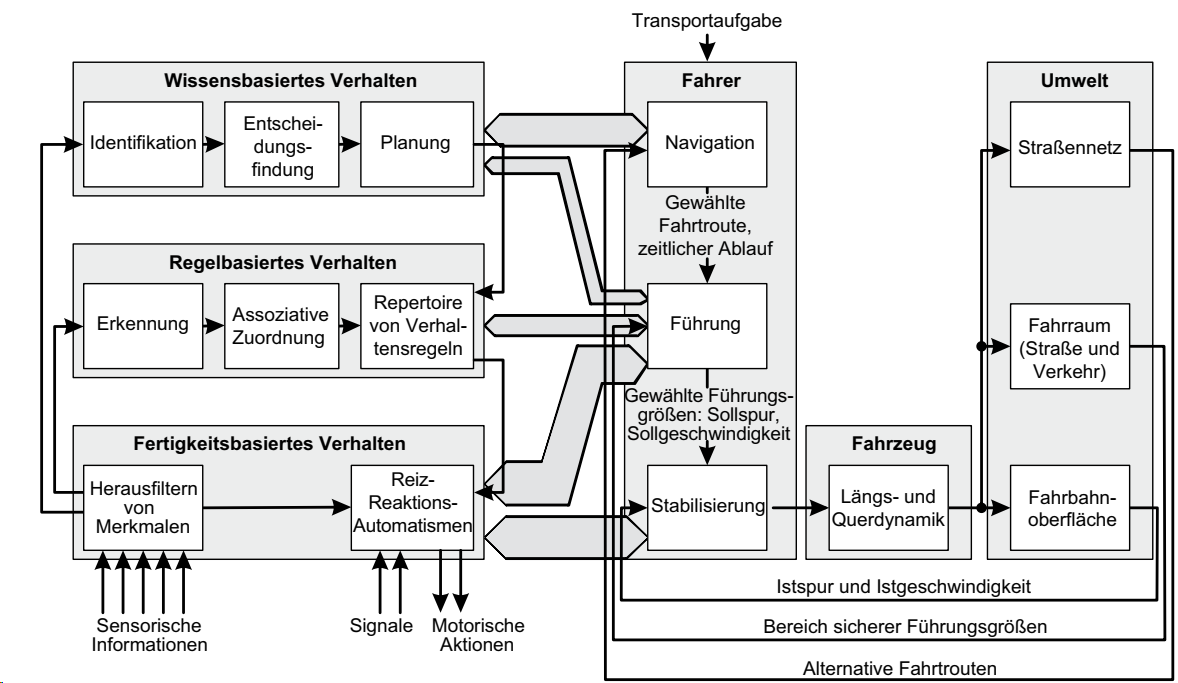
\includegraphics[width=1\textwidth]{images/related_work/Modell_Rasmussen.png}
    \caption{Gegenüberstellung von Drei-Ebenen-Modell für zielgerichtete Tätigkeiten des Menschen und Drei-Ebenen-Hierarchie der Fahraufgabe}
    \label{fig:rasmussen}
    \medskip
    {\footnotesize Quelle: Abbildung übernommen aus
    \cite[S.~19]{donges2015fahrerverhaltensmodelle}.}
\end{figure}

Geisler \cite{Geisler_hci2021} unterteilt nach Rasmussen \cite{Rasmussen1983} das menschliche Fahrverhalten in drei Ebenen. Abbildung \ref{fig:rasmussen} zeigt die Gegenüberstellung von Verhaltensweisen des Menschen und Fahraufgaben. Der Forscher konstatiert, dass sich die Verhaltensarten im wesentlichen anhand des Ausmaßes der kognitiven Belastung unterscheiden \cite{Geisler_hci2021}. Während das fertigkeitsbasierte Verhalten unbewusst und als reines Reiz-Reaktions-Schema ablaufe, könne die fahrzeugführende Person beim regelbasierten Verhalten immerhin noch auf sequentiell verknüpfte Schritte zurückgreifen, während das wissensbasierte Verhalten ein bewusstes Überlegen erfordere, so Geisler \cite{Geisler_hci2021}. Desweiteren könnten durch Training und Erfahrung die kognitive Belastung reduziert werden, was zu geringeren Reaktions- und Ausführungszeiten sowie geringerer Ablenkung führe \cite{Geisler_hci2021}. Der Forscher schließt, dass Lernförderlichkeit und Sicherheit des Systems eng miteinander verknüpft seien \cite{Geisler_hci2021}.

Für diese Forschungsarbeit bedeutet dies, dass ein Onboarding für Assistenzsysteme den Anteil an kognitiv fordernden Prozessen möglichst minimieren sollte. Fahrer*innen sollten insbesondere in unübersichtlichen Situationen einzelne Hinweise von Assistenzsystemen schnell zuordnen und wiedererkennen können, ohne, aus Sicht der Fahrzeugsicherheit, lange und damit ungünstige Überlegungen durchführen zu müssen. Außerdem sollte bei Assistenzsystemen, welche möglicherweise seltener zum Einsatz kommen, ein ausführlicheres Onboarding stattfinden, da die Fahrer*innen auf weniger Erfahrungen zurückgreifen können.  

\section{Human Factors bei der Nutzung von Fahrassistenzsystemen}
\label{sec:human_factors}

\subsection{Wahrnehmung, Aufmerksamkeit und Situationsbewusstsein}
\label{subsec:wahrnehmung_situationsbewusstsein}
abc

\subsection{Mentale Modelle und Mode Awareness}
\label{subsec:mentale_modelle}
abc

\subsection{Vertrauen, Reliance und Akzeptanz}
\label{subsec:vertrauen_akzeptanz}
abc

\subsection{Lernen und Anpassung an Fahrassistenzsysteme}
\label{subsec:lernen_anpassung}
abc


\section{Defizite der gegenwärtigen Informationsvermittlung}
\label{sec:informationsdefizite}

\subsection{Fehlvorstellungen und nicht intendierte Nutzung}
\label{subsec:fehlvorstellungen_fehlgebrauch}
abc

\subsection{Fahrzeughandbücher, Fahrzeugkauf und Fahrausbildung}
\label{subsec:informationsquellen}
abc

\subsection{Kommunikation von Systemfähigkeiten und Systemgrenzen}
\label{subsec:kommunikation_systemgrenzen}
abc

\subsection{Anforderungen an die Fahrer*innenbildung}
\label{subsec:anforderungen_fahrerbildung}
abc


\section{Training und Onboarding für Fahrassistenzsysteme}
\label{sec:training_onboarding}

\subsection{Begriffsverständnis und Ziele des Onboardings}
\label{subsec:onboarding_begriff}
abc

\subsection{Lerninhalte eines Onboardings}
\label{subsec:onboarding_lerninhalte}
abc

\subsection{Zeitpunkt und Nutzungskontext der Informationsvermittlung}
\label{subsec:onboarding_zeitpunkt}
abc

\subsection{Vermittlungsformen und Interaktionskonzepte}
\label{subsec:onboarding_vermittlungsformen}
abc

\subsection{Motivation, Personalisierung und adaptive Unterstützung}
\label{subsec:onboarding_adaptivitaet}
abc

\subsection{Empirische Befunde zur Wirksamkeit}
\label{subsec:onboarding_wirksamkeit}
abc


\section{Partizipative Entwicklung von In-Car-Onboardings}
\label{sec:partizipative_entwicklung}

\subsection{Grundlagen des partizipativen Designs}
\label{subsec:grundlagen_partizipatives_design}
abc

\subsection{Nutzer*innen als Expert*innen ihrer Nutzungserfahrungen}
\label{subsec:nutzende_expertinnen}
abc

\subsection{Überführung von Nutzer*innenbedarfen in Gestaltungsanforderungen}
\label{subsec:anforderungsableitung}
abc


\section{Evaluation von Onboardings für Fahrassistenzsysteme}
\label{sec:evaluation_onboarding}

\subsection{Evaluationskriterien und Zielgrößen}
\label{subsec:evaluationskriterien}
abc

\subsection{Erfassung mentaler Modelle und Systemverständnis}
\label{subsec:messung_mentale_modelle}
abc

\subsection{Verhaltens- und leistungsbezogene Evaluation}
\label{subsec:verhaltensmessung}
abc

\subsection{Fahrsimulatoren als Evaluationsumgebung}
\label{subsec:fahrsimulator}
abc


\section{Synthese des Forschungsstands und Forschungslücke}
\label{sec:synthese_forschungsluecke}